%%%%%%%%%%%%%%%%%%%%%%%%%%%%%%%%%%%%%%%%%%%%%%%%%%%%%%%%
%%%%%%%%%%%%%%%%%%%%%%%%%%%%%%%%%%%%%%%%%%%%%%%%%%%%%%%%
\section{Results}
\label{sec:results}
%%%%%%%%%%%%%%%%%%%%%%%%%%%%%%%%%%%%%%%%%%%%%%%%%%%%%%%%
%%%%%%%%%%%%%%%%%%%%%%%%%%%%%%%%%%%%%%%%%%%%%%%%%%%%%%%%
%
%%%%%%%%%%%%%%%%%%%%%%%%%%%%%%%%%%%%%%%%%%%%%%%%%%%%%%%%
\subsection{Flood Mapping Performance}
\label{ssec:flood_mapping_performance}
%%%%%%%%%%%%%%%%%%%%%%%%%%%%%%%%%%%%%%%%%%%%%%%%%%%%%%%%
%
We produced FIMs for the entire BLE domain within the 49 HUC8 areas across several states in the south central US. 
The forecasted FIMs using the discharges for the 1\% (100 year) and 0.2\% (500 year) recurrence flows directly from HEC-RAS were used to avoid noise and errors from hydrological processes.
We computed the statistics, CSI, POD, and FAR, for both 100 and 500 year events for Mannings N set to 0.06 and 0.12.
These results are presented in Figure \ref{fig:violin_plot} as violin plots and in Table \ref{tab:aggregate_metrics} as aggregated metrics with the results for MS and GMS presented as percentage changes from their respective FR values.
To be more specific, Table \ref{tab:aggregate_metrics} sums the primary metrics, TP, FP, FN, and TN, across all HUC8s then recomputes the secondary metrics which was done to better account for large variances in HUC8 size.
The same trends discussed below are consistent across both reporting methods (Figure \ref{fig:violin_plot} and Table \ref{tab:aggregate_metrics}).

The distribution of these flood extent metrics can be examined in Figure \ref{fig:violin_plot} as violin plots.
Each half of a violin plot represents the kernel density estimation (KDE) for a given model (FR, MS, GMS), given Manning's n value (0.06, 0.12), and given recurrence interval (1\%, 0.2\%), and performance metric (CSI, POD, FAR).
For example, let's examine the violin plot for the row marked CSI and column for Manning's n = 0.06.
This sub-figure shows the CSI distributions across all 49 HUC8s when Manning's n is set to 0.06.
Each independent, whole violin represents the distribution of FR, MS, or GMS while each half of the violin represents the distribution of that data divided up by magnitude (blue for 100 yr and orange for 500 yr).
The horizontal dashed and dotted lines represent the 25th, 50th, and 75th percentiles from bottom to top, respectively.
Additionally, we show trend lines symbolized in green that for each metric and Manning's n combination denotes the best fit line for the three methods (FR, MS, and GMS).
To avoid having two trend lines per sub-figure, we elected to aggregate the two magnitudes together as they tend to observe similar trends across the three models.
The slope of each trend line is quantified in the figure by its $\beta_1$ value and the p-value for that statistic which tests the significance of that trend (deviation from a zero sloped trend line).

% Interpretation of metrics
Both Figure \ref{fig:violin_plot} and Table \ref{tab:aggregate_metrics} contain a fair amount of information that is central to the objectives of this study.
As previously stated in Section \ref{ssec:evaluation}, we consider CSI as a general proxy for the skill of the inundation extents with POD denoting skill on inundated areas and FAR indicating skill on non-inundated areas.
Again, the main objective of the study is to introduce how computing HAND with disaggregated stream networks to those with unit stream order can enhance the fidelity of FIMs by capturing fluvial inundation from multiple sources as opposed to that of just the nearest drainage line.
As can be seen in Figure \ref{fig:violin_plot} and Table \ref{tab:aggregate_metrics}, CSI generally increases from FR to MS and MS to GMS for both sets of Manning's n values and flood magnitudes.
This increase is primarily driven by an increase in POD thus generally increasing the probability of correctly detecting inundation.
Also, we note that FAR is somewhat, albeit marginally, decreased from FR to MS and MS to GMS for both sets of Manning's n values and flood magnitudes.
The increases in CSI and POD as well as the decreases in FAR with respect to the methods, FR, MS, and GMS, are not only observed among the trend lines but also in the 25th, 50th, and 75th percentiles (Figure \ref{fig:violin_plot}).
So overall and in other words, the entire distribution of HUC8s improves across the three methods.
Due to the means by which FIM is produced utilizing FR, MS, and GMS, we can say that the more we derive HAND on networks of unit stream order and mosaic the resulting FIMs, the better those FIMs perform.
We move more details on the relationship between stream order and FIM skill to the Discussion section (Section \ref{sec:discussion}).

Additional noteworthy trends in Figure \ref{fig:violin_plot} center around the all-around better performance of FIMs for those of higher Manning's n values and recurrence flows.
The higher Manning's n value enhances performance for both recurrence intervals across all models which seems to better agree with the value used in the BLE model, 0.11 \cite{fema2021base,fema2021estimated}.
Most of this improvement is driven by significant increases in POD but, unfortunately, leading to a significant amount of over-prediction as observed by the increase in FAR.
More work can be invested to better regionalize Manning's n values for FIM purposes with HAND.
We also observe additional trends associated with the magnitude or recurrence interval of the flow rates used with the higher flow rates exhibiting better overall CSI, POD, and FAR values than the lower, 100 yr magnitude.
We introduce in the Discussion (Section \ref{sec:discussion}) that this skill premium exhibited by higher flow events could be due higher quality elevation data in regions that are not described as bathymetric areas.
%
\begin{figure}[H]
\centering
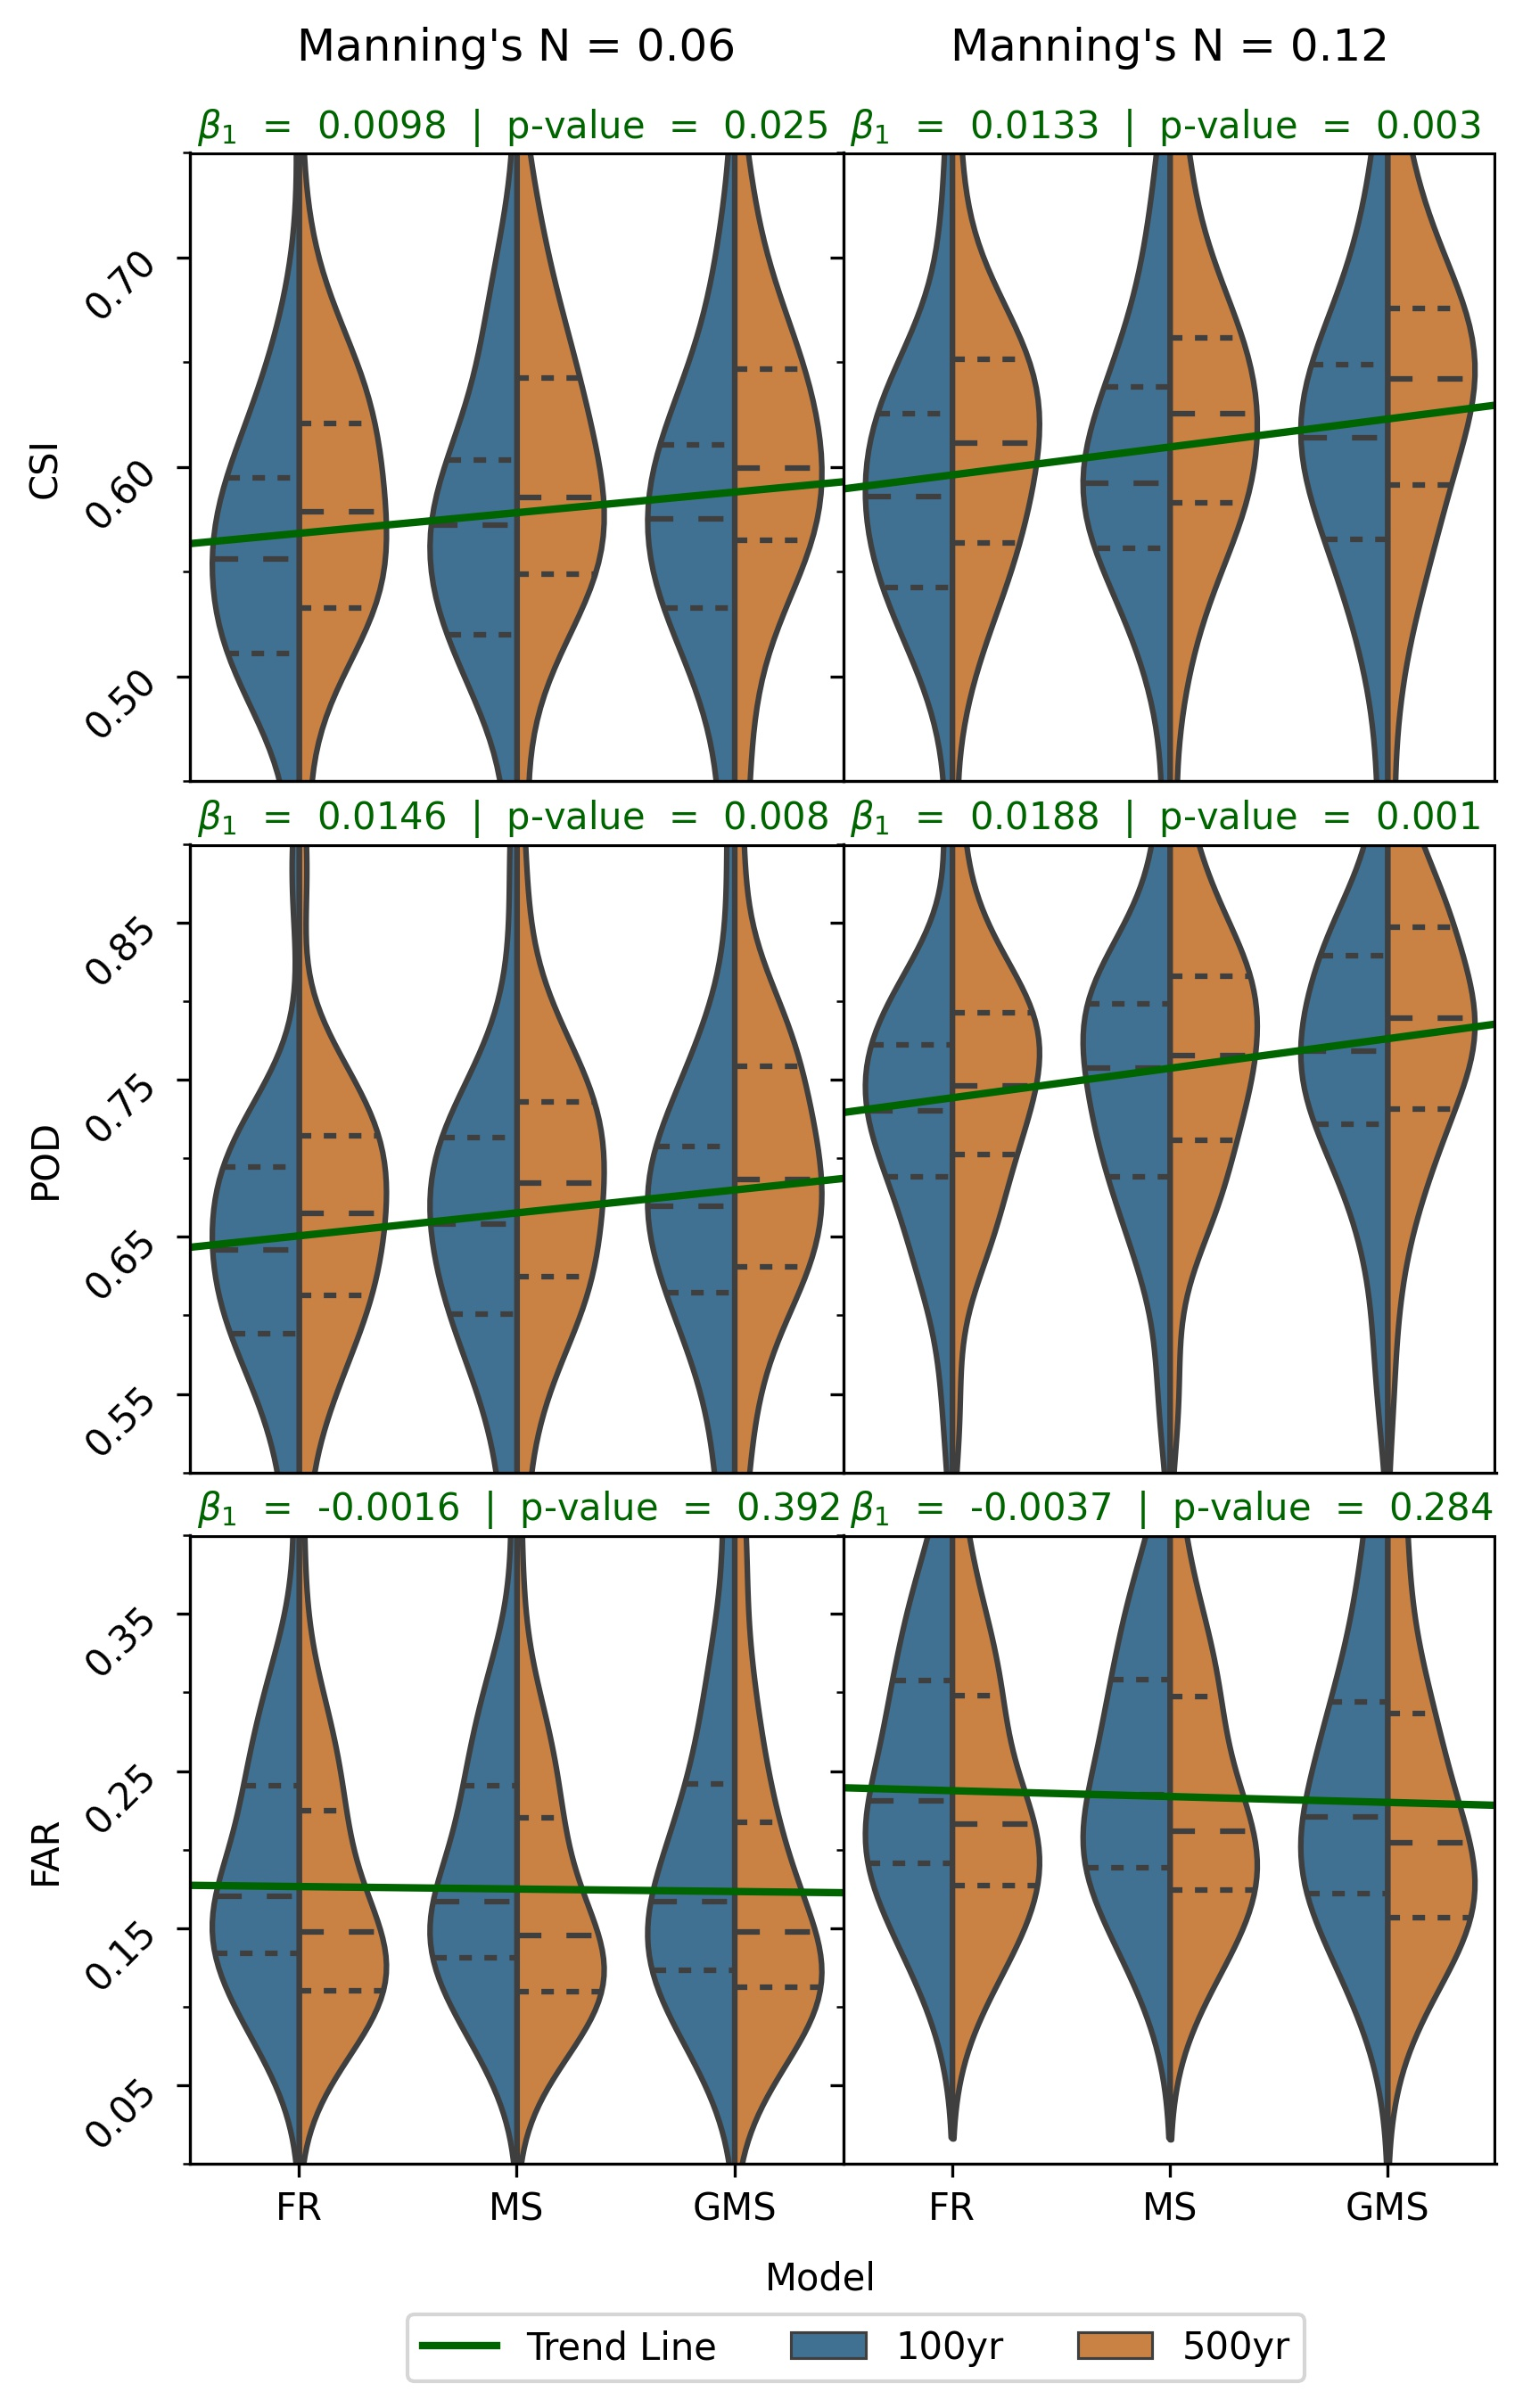
\includegraphics[scale=0.9]{figures/violin_plots.jpg}
\caption{Shows kernel density estimation of the distributions (sample size = 49) for 1\% (100 year) and 0.2\% (500 year) along with horizontal, dashed lines for the 25th, 50th, and 75th percentiles (in order from bottom to top).
The sub-figures separate the combination of three metrics (CSI, POD, and FAR) for two settings of Manning's n (0.06 and 0.12).
Trend lines for each metric - Mannings combination are shown (sample size = 294) along with associated slope and p-value of slope testing one-tailed significance.}
\label{fig:violin_plot}
\end{figure}
%
\begin{table}[H]
\caption{ Recomputed CSI, POD, and FAR using the primary metrics, TPs, FPs, and FNs, aggregated to the BLE domain.
         The values for MS and GMS methods are expressed in percentage change (\%) from their respective values with the same Manning's n, magnitude, and metric combination in the Full Resolution (FR) method columns.
         The best value across models is highlighted in bold.}
\label{tab:aggregate_metrics}
\centering
%\begin{tabular}{|p{2cm}|p{2cm}|p{2cm}|p{2cm}|}
\begin{tabular}{|c|c||c|c|c|c|c|c|}
\hline
\multirow{2}{*}{Metric} & \multirow{2}{*}{Manning's n} & \multicolumn{2}{|c|}{FR} & \multicolumn{2}{|c|}{\shortstack{MS\\(\% Change)}} & \multicolumn{2}{|c|}{\shortstack{GMS\\(\% Change)}} \\
\cline{3-8}
  &  & 100 yr & 500 yr & 100 yr & 500 yr & 100 yr & 500 yr \\
\hline
\multirow{2}{*}{CSI} & 0.06 & 0.5576 & 0.5839 & 2.53 & 2.59 & \textbf{3.95} & \textbf{4.04} \\
\cline{2-8}
  & 0.12 & 0.5915 & 0.6149 & 2.35 & 2.26 & \textbf{4.51} & \textbf{4.65} \\
\hline
\multirow{2}{*}{POD} & 0.06 & 0.6354 & 0.6575 & 2.68 & 2.74 & \textbf{4.39} & \textbf{4.38} \\
\cline{2-8}
  & 0.12 & 0.7255 & 0.7446 & 2.83 & 2.71 & \textbf{4.84} & \textbf{4.89} \\
\hline
\multirow{2}{*}{FAR} & 0.06 & 0.1800 & 0.1609 & -0.72 & \textbf{-1.24} & \textbf{-1.22} & \textbf{-1.24} \\
\cline{2-8}
  & 0.12 & 0.2379 & 0.2208 & -0.21 & -0.18 & \textbf{-2.31} & \textbf{-2.72} \\
\hline
\end{tabular}
\end{table}
%
%%%%%%%%%%%%%%%%%%%%%%%%%%%%%%%%%%%%%%%%%%%%%%%%%%%%%%%%
\subsection{Computational Performance}
\label{ssec:compuational_performance}
%%%%%%%%%%%%%%%%%%%%%%%%%%%%%%%%%%%%%%%%%%%%%%%%%%%%%%%%
%
The NFIE experiments were able to produce HAND for 331 HUC6's in 1.34 CPU years \cite{liu2016cybergis} and estimates using work from \citeA{djokic2019arc} put producing HAND at the FR NWM at 0.55 CPU years. 
For our work, we were able to produce HAND at the full NWM resolution in 0.13 CPU years which represents a substantial speed-up compared to previous works.
For the MS resolution an additional, 0.05 CPU years is required on top of this bringing the total to about 0.18 CPU years to produce 2,188 HUC8s that span additional areas not covered in previous HAND versions including Hawaii and Puerto Rico.
GMS which generalizes HAND production to the LP scale adds a significant amount of CPU time to the process bringing the estimate total to about 1.17 CPU years.
%
